\section{Transduction}

\begin{figure}[H]
    \centering
    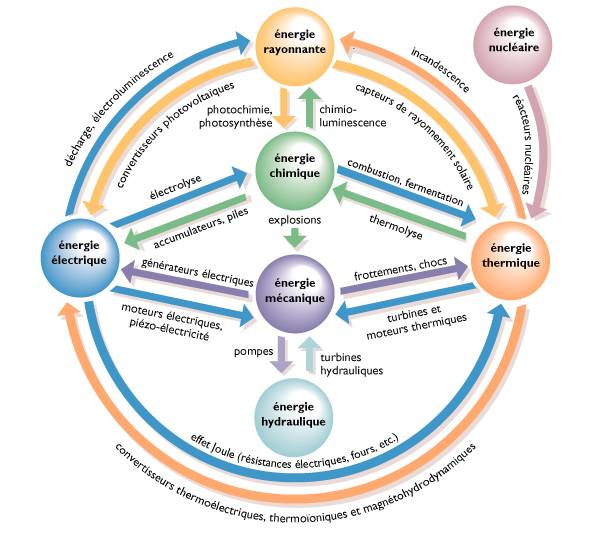
\includegraphics[width = 0.6\textwidth]{L2/img/energy.jpg}
\end{figure}

\begin{mydef}
A transduction is a conversion of energy from one domain to another.
\end{mydef}

Energy manifests itself through parameters (wavelength for light, temperature for thermal, \dots).
Transduction is a generic term for :
\begin{itemize}
    \item Sensing: detecting one or more parameters
    \item Actuation: acting on one or more parameters
\end{itemize}

\begin{mydef}
A transducer is a device that performs any kind
of transduction.
\end{mydef}

A transduction can be reversible or not. \textbf{Electricity} is also a physical signal!

Two kinds of sensing:

\begin{itemize}
    \item Direct: converts a stimulus into an electrical signal or modifies an electrical signal by using an appropriate physical effect (i.e. piezoelectric components).
    \item Indirect: complex sensors need one or more transducers of energy before a direct sensor can be employed to generate an electrical output (i.e. a microphone, air pressure waves induce mechanical displacement of a membrane that itself induces an EM field in a coil).
\end{itemize}

It is necessary to make a distinction between \textbf{counting} and \textbf{measuring}:

\begin{mydef}
Measuring compares a signal with a reference value on
a given scale (continuous, analog).
\end{mydef}

\begin{mydef}
Counting is enumerating (discrete, digital).
\end{mydef}

For a digitized measurement, we first measure a signal and then convert it for counting.

\subsection{Capacitive sensors}

Capacitance is obtained by an AC current excitation and reads as an impedance. For measurements, we can measure \textbf{topological changes} (distance) or \textbf{dielectric changes} (permittivity), but \textbf{never both}.

\subsubsection{Topology changes}

\begin{itemize}
    \item Plate capacitor: $ C = \frac{\epsilon_r \epsilon_0 A}{d} \rightarrow$ non-linear with respect to $d$
    \item Cylindrical capacitor: $C = \frac{2\pi \epsilon_r \epsilon_0 l}{\ln(b/a)} \rightarrow$ linear with respect to $l$
\end{itemize}

\begin{figure}[H]
    \centering
    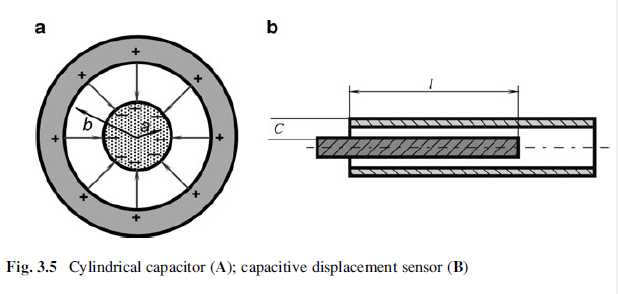
\includegraphics[width = 0.6\textwidth]{L2/img/capa-cylindrique.PNG}
\end{figure}

\subsubsection{Dielectric changes}

In a good capacitor used in electronic circuits, a dielectric constant $k$ and
geometry $G$ must be stable. Ideally, they should not vary with temperature,
humidity, pressure, or any other environmental factors. It is the opposite as regards the capacitive sensors. If you want to design a \textbf{good capacitive} sensor, you need to make a \textbf{bad capacitor}, whose
value varies with temperature, or humidity, or pressure, or whatever it is needed to
sense.

For example, we can measure water level with a cylindrical capacitor (the capacitance will change with the water level, as it will modify the dielectric constant\footnote{We need to pay attention to short circuits.}). However, since the water dielectric constant depends on temperature, this system will need to be coupled with a temperature sensor to compensate this dependence.
\begin{figure}[H]
    \centering
    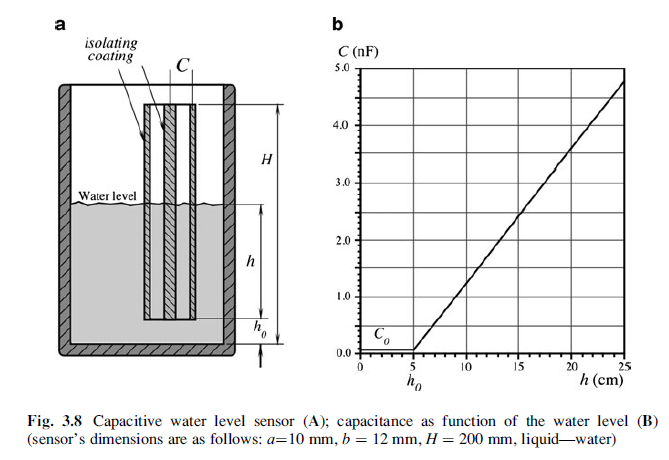
\includegraphics[width = 0.6\textwidth]{L2/img/water-level.PNG}
\end{figure}

\subsection{Magnetic sensors}

\subsubsection{Magnetism}

\begin{itemize}
    \item Magnets are used as position sensors and/or presence detector
    \item Inductors are used as position sensors
    \item Magnetic forces are used for the indirect currents detection
\end{itemize}

\subsubsection{Hall effect}

\begin{minipage}{0.5 \linewidth}

Nowadays, Hall sensors are used to detect magnetic fields,
position, and displacement of objects. The effect is based on the interaction between moving electric carriers and an
external magnetic field. By measuring the transverse voltage (transverse Hall potential difference $V_H$) when a known control voltage is applied, we can determine the magnetic field $B$.

\end{minipage}\hfill
\begin{minipage}{0.5 \linewidth}
\begin{figure}[H]
    \centering
    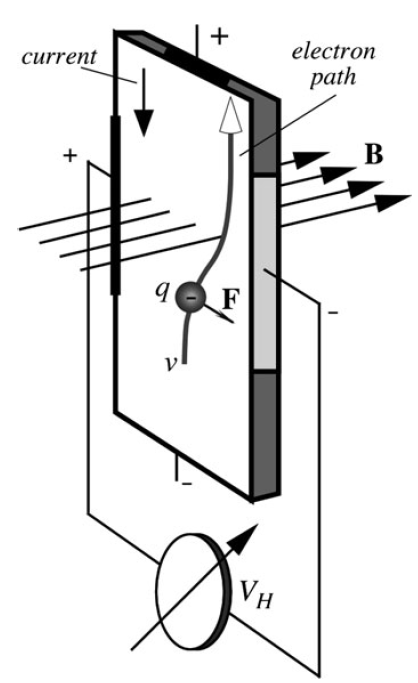
\includegraphics[width = 0.4\textwidth]{L2/img/hall.PNG}
\end{figure}
\end{minipage}

\subsection{Resistive sensors}

General principle:
\[
    R = \frac{\rho l}{a}
\]
Once again, a good resistor is one that will remain stable : its parameters do not change much with external conditions. Therefore, for sensing applications, we look for \textbf{bad resistors}. 

With a resistor, we can sense:
\begin{itemize}
    \item Temperature
    \item Strain
    \item Moisture
    \item Electricity
\end{itemize}

\subsubsection{Thermistors}

\paragraph{Resistance Temperature Detector (RTD)}
RTD are composed of pure metals with $\alpha > 0$, they operate over large temperature range. For low accuracy applications, the following equation can be used:
\[
    \rho = \rho_0 \left(1 + \alpha \frac{T - T_0}{T_0}\right)
\]
When more accuracy is needed, we can use a second order model, such as the following:
\[
    \rho = 4.45 + 0.0269\:T + 1.914\cdot 10^{-6}\:T^2
\]

\paragraph{Positive Thermal Coefficient (PTC) \& Negative Thermal Coefficient (NTC)}

Same principle than RTD but made with conductive ceramics (oxides),
doped semiconductors, polymers.
$\alpha > 0$ for PTC and $\alpha < 0 $ for NTC. 

\textbf{Quick example :} having $\alpha = \SI{2}{[\celsius^{-1}]}$ means that the change in resistance value is 200\% per $\celsius$.   

\textbf{Advantages}: cheaper than RTD and more precise for a certain range of temperature.

The model used for the resistance of a semiconductor is the Steinhart-Hart model, which is the following:
\[
    \dfrac{1}{T} = a + b \ln(R) + c\ln(R)^3
\]
where $a,b,c$ are the Steinhart-Hart coefficients, depending on the type and model of the used thermistor. 

For NTC, $\alpha = \frac{1}{R} \frac{\Delta R}{\Delta T} = - \dfrac{\beta}{T^2}$ ($\beta$ is the characteristic temperature).

\subsubsection{Piezoresistivity}

Piezo-resistive effect: electrical resistance changes when the material is mechanically deformed $\rightarrow$ used in beams to see if dimensions are changing (bridge, buildings, \dots).
$$ \frac{\Delta R}{R} = S_e e $$
The factor $e$ is called strain, which is a
normalized deformation of the material. $S_e$ is known as the gauge factor or sensitivity of the strain gauge element.

Applying strain on a cylindrical rod is equivalent to increasing its length $l$ and reducing its section $a$. This induces a $\Delta R$, according to the relation : 
$$R = \frac{\rho l}{a}$$

\subsubsection{Hygristor}

A hygristor is a moisture dependent resistor. It can be fabricated of a hygroscopic material whose
specific resistivity is strongly influenced by concentration of the absorbed water
molecules.

\subsection{Piezoelectric sensors}

The piezoelectric effect is generation of electric charge by a crystalline material
upon subjecting it to stress. The effect exists in natural crystals, such as quartz
(chemical formula $SiO_2$), and poled (artificially polarized) human-made ceramics
and some polymers.

Piezoelectricity is found in useful applications, such as the production and detection of sound, generation of high voltages, electronic frequency generation, microbalances, ignition source for cigarette lighters, as well as the time reference source in quartz watches. 

\begin{figure}[H]
    \centering
    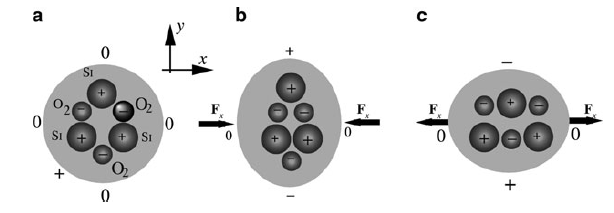
\includegraphics[width = 0.6\textwidth]{L2/img/piezo.PNG}
\end{figure}

Piezoelectricity is synthesized through the following equations : 
$$S_{ij} = s_{ijkl}^E T_{kl} + d_{kij} E_k$$
$$D_i = d_{ikl} T_{kl} + \epsilon_{ik}^T E_{k}$$

where : 
\begin{itemize}
    \item $S_{ij}$ is the mechanical strain field,
    \item $s_{ijkl}^E$ is the elastic compliance, tensor
    \item $T_{kl}$ mechanical stress field ($\approx$ stress tensor),
    \item $E_k$ is the electrical field,
    \item $D_i$ is the electrical displacement field,
    \item $d_{ikl}$ is the piezoelectric tensor,
    \item and $\epsilon_{ik}^T$ is the dielectric permittivity tensor.
\end{itemize}
All these equations can be synthesized in a matrix, linking strain and electrical displacement to mechanical stress and electric field. The mechanical, electrical and piezoelectric terms are placed as on the figure below.
\begin{figure}[H]
    \centering
    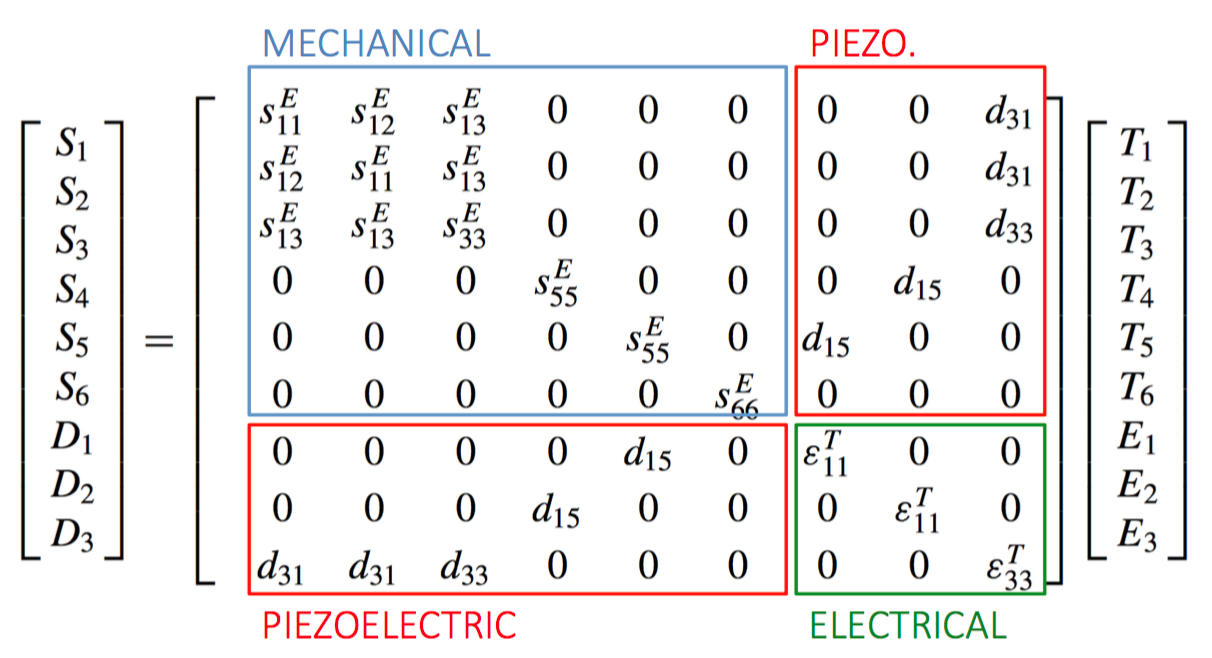
\includegraphics[width = 0.6\textwidth]{L2/img/pizzo}
\end{figure}

Piezoelectric materials can however be described in much simpler terms, in particular with their coupling coefficient : 
$$k^2 = \frac{\text{converted energy}}{\text{input energy}}$$
